\documentclass{article}

\usepackage{amsmath}
\usepackage{amssymb}
\usepackage{parskip}
\usepackage{fullpage}
\usepackage{graphicx}
\usepackage{hyperref}
\usepackage{listings}
\usepackage{xcolor}
\usepackage{wrapfig}
\usepackage{tikz}
\usetikzlibrary{lindenmayersystems}

\hypersetup{
    colorlinks=true,
    linkcolor=black,
    urlcolor=blue,
    pdftitle={Paolo Bettelini - Diaries},
    pdfpagemode=FullScreen,
}

\newcommand{\wrapfill}{
    \par
    \ifnum \value{WF@wrappedlines} > 0
        \addtocounter{WF@wrappedlines}{-1}%
        \null\vspace{
            \arabic{WF@wrappedlines}
            \baselineskip
        }
        \WFclear
    \fi
}

\definecolor{background}{HTML}{EEEEEE}

\lstdefinestyle{generic} {
    backgroundcolor=\color{background},
    numbers=none,
    basicstyle=\ttfamily\color{black},
    breaklines=true,
    frame=lines
}

\title{%
    Lindenmayer's Garden \\
    \phantom{} \\
    \large Scuola d'Arti e Mestieri di Trevano (SAMT) \\
    \large Diaries
}

\author{Paolo Bettelini}

\date{}

\pgfdeclarelindenmayersystem{A}{
  \rule{V -> [+++W][---W]YV}
  \rule{W -> +X[-W]Z}
  \rule{X -> -W[+X]Z}
  \rule{Y -> YZ}
  \rule{Z -> [-FFF][+FFF]F}
}

\begin{document}

%\begin{tikzpicture}[rotate=90]
%    \draw
%        [purple!50!black,thin,line cap=round]
%        l-system [l-system={A,axiom=VZFFF
%        ,order=8,angle=20,step=0.2cm}];
%\end{tikzpicture}

\begin{minipage}{0.55\textwidth}
    \maketitle
\end{minipage}
\begin{minipage}{0.45\textwidth}
    \vspace*{3cm}
    
\begin{tikzpicture}[rotate=90]
        \draw
            [purple!50!black,thin,line cap=round]
            l-system [l-system={A,axiom=VZFFF
            ,order=8,angle=20,step=0.25cm}];
    \end{tikzpicture}
\end{minipage}

\vspace*{1cm}

\tableofcontents

\pagebreak

\section{Working Sessions}

\subsection{2023-05-02}

Work hours:\\
\textbf{08:30 - 10:30}: Initial analysis \\
\textbf{10:30 - 11:25}: Repository setup

Today I read time the requirements for the project for the first.
I thoroughly analyzed each requirements with my advisor, with whom, after a long discussion,
we decided to drastically change. \\
The initial premise and functionality of the project does remain the same, but it will be
executed with a wider approach, which both augments its functionality and simplifies its workings.

In the second half of the working session I setup the repository with the initial files, folder and documents.

The plan for the next working session is to create the Gantt chart.

\subsection{2023-05-03}

Work hours:\\
\textbf{09:05 - 10:00}: Requirements \\
\textbf{10:00 - 10:15}: Documentation \\
\textbf{10:15 - 10:35}: Initial Gantt Chart \\
\textbf{10:50 - 12:10}: Use Cases \\
\textbf{13:20 - 13:50}: UI Design \\
\textbf{13:50 - 14:10}: Uses Cases \\
\textbf{14:10 - 14:45}: \texttt{lsystems-engine} \\
\textbf{15:05 - 15:40}: \texttt{lsystems-renderer} \\
\textbf{15:40 - 16:20}: \texttt{lsystems-gui}

Today I started adding content to the documentation.
I wrote the requirements of the project and some other minor section.

I created the following sections:
\begin{itemize}
    \item \texttt{Introduction.Information}
    \item \texttt{Analysis.Requirements}
    \item \texttt{Analysis.Use Cases}
    \item \texttt{Analysis.GUI Design}
\end{itemize}

The \texttt{Technologies.Rust} section was recycled from a previous
project.

In the second half of the working session I drew the UI design sketch
and started coding.

I plan to structure the project with the following crates:
\begin{itemize}
    \item \texttt{lsystems-engine}: Basic L-System string expansion
    \item \texttt{lsystems-renderer}: Rendering logic with abstract operations
    \item \texttt{lsystems-parser}: Config parser for \texttt{lsystems-renderer}
    \item \texttt{lsystems-cairo}: Rendering implementation for \texttt{cairo}
    \item \texttt{lsystems-gui}: Graphical User Interface
\end{itemize}

I created the \texttt{lsystems-engine} lib and
implemented the basic L-systems string expansion.
I also added a unit test to make sure the string is expanded correctly.

I created the \texttt{lsystems-renderer} lib and
started sketching the library structure and

I created \texttt{lsystems-gui} and
setup a simple GTK4 application to make sure everything is ready.

I am ahead of the initial planning.

\textbf{Git status}:
\begin{enumerate}
    \item Created \texttt{gui} branch
    \item Created \texttt{renderer} branch
\end{enumerate}

\subsection{2023-05-04}

Work hours:\\
\textbf{08:20 - 08:40}: Renderer abstraction \\
\textbf{08:40 - 09:50}: Renderer implementation \\
\textbf{10:05 - 11:25}: Fractal drawing

Today I created the rendering abstraction
and wrote a basic implementation of the fractal drawing.

To achieve this I needed to implement the drawing abstraction for \texttt{cairo-rs}.

I hardcoded a fractal renderer into the code and tried to draw it.
Something resembling the fractal is renderer onto the canvas,
but it is still broken.

The plan for the next working session is to render the fractal correctly
and continue the documentation.

I am still ahead planning.

\textbf{Git status}:
\begin{enumerate}
    \item Merged \texttt{gui} into \texttt{master}
    \item Merged \texttt{renderer} into \texttt{master}
    \item Created \texttt{parser} branch
    \item Created \texttt{fractal-drawing} branch
\end{enumerate}

\pagebreak

\subsection{2023-05-05}

Work hours:\\
\textbf{08:20 - 08:50}: Fixed fractal drawing \\
\textbf{08:50 - 10:40}: Parser implementation \\
\textbf{10:40 - 11:20}: Fractal from file \\
\textbf{13:35 - 14:35}: Documentation

Today I implemented the parser for the fractal configuration.
The parser is not ready but it is stable enough and supports the most part
of the basic grammar.

The program is now able to read a file containing the fractal specifications
and then render it.

The file looks like the following:

\begin{figure}[h]
\begin{minipage}{0.5\textwidth}
    \begin{lstlisting}[basicstyle=\ttfamily]
        LINE = 10
        ANGLE = 0.62832
    
        F -> F[+FF][-FF]F[-F][+F]F
    
        axiom F
        iter 5
        initial_pos 375,750
    
        F: forward LINE
        +: rotate ANGLE
        -: rotate -ANGLE
        [: push
        ]: pop
    \end{lstlisting}
\end{minipage}
\begin{minipage}{0.5\textwidth}
    
\includegraphics[width=\textwidth]{fractal.png}
\end{minipage}
\end{figure}

\textbf{Git status}:
\begin{enumerate}
    \item Merged \texttt{fractal-drawing} into \texttt{master}
    \item Merged \texttt{parser} into \texttt{master}
\end{enumerate}

In the second half of the working session I continued the documentation.

I modified or created the following sections:
\begin{itemize}
    \item \texttt{Technologies.GTK4}
    \item \texttt{L-Systems.Definition}
    \item \texttt{L-Systems.Examples}
\end{itemize}

\pagebreak

\subsection{2023-05-08}

Work hours:\\
\textbf{09:05 - 12:30}: GUI editor \\
\textbf{13:15 - 14:45}: Stochastic behavior \\
\textbf{15:00 - 16:20}: Generic improvements

Today I implemented the first version of the GUI editor.
When the application starts, some textboxs are loaded
with the default lines of a fractal configuration.
By changing the content of the textboxs the fractal is updated in real-time.

In the second half of the working session I implemented
the stochastic behavior, namely the \texttt{rand(lower, upper)} function
and the \texttt{seed} command.

The following image illustrates such behavior.

\begin{center}
    \begin{figure}[h]
        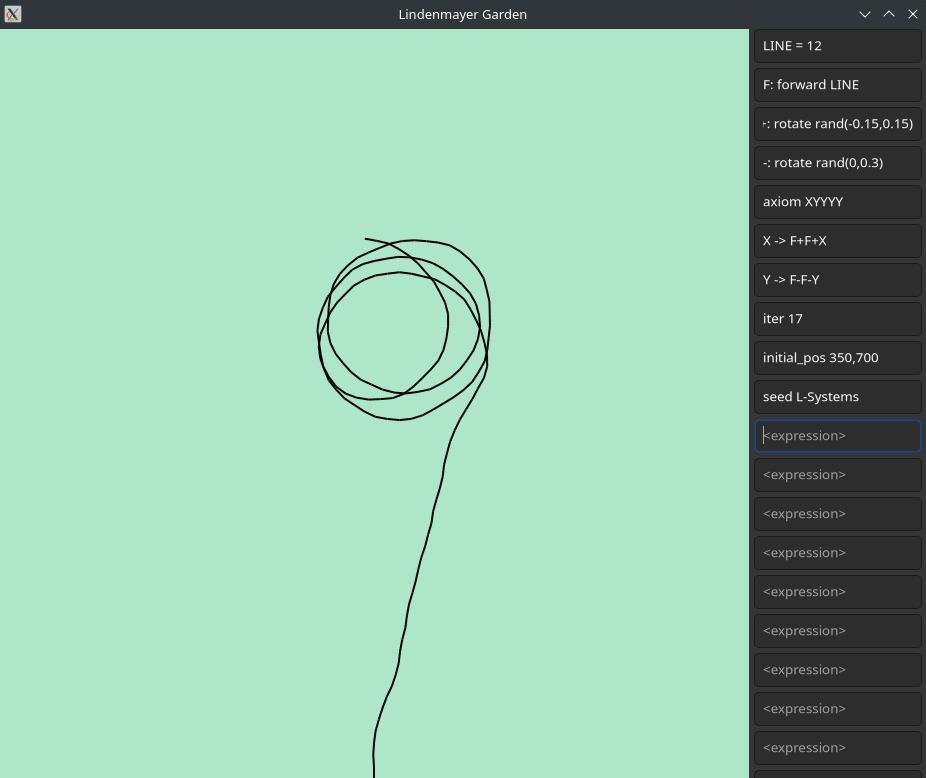
\includegraphics[width=0.8\textwidth]{fractal_rand.png}
    \end{figure}
\end{center}

\textbf{Git status}:
\begin{enumerate}
    \item Created \texttt{gui-editing} branch
    \item Merged \texttt{gui-editing} into \texttt{main}
    \item Created \texttt{stochastic} branch
    \item Merged \texttt{stochastic} into \texttt{main}
    \item Created \texttt{development} branch (generic improvements and fixes)
\end{enumerate}

\pagebreak

\subsection{2023-05-09}

Work hours:\\
\textbf{08:30 - 09:00}: Ignore feature \\
\textbf{09:00 - 09:50}: Thickness feature \\
\textbf{10:20 - 11:15}: Generic improvements and features \\
\textbf{11:15 - 11:30}: Logging

Today I implemented the \textbf{ignore} and \textbf{thickness} features.

The ignore feature implements a command to ignore the next \(N\) symbols
in the string. \\
I found the symbol defined as \texttt{!: ignore rand(0,1.05)} very useful
to give some trees a more natural growth.
Here's an example

\begin{center}
    \begin{figure}[h]
        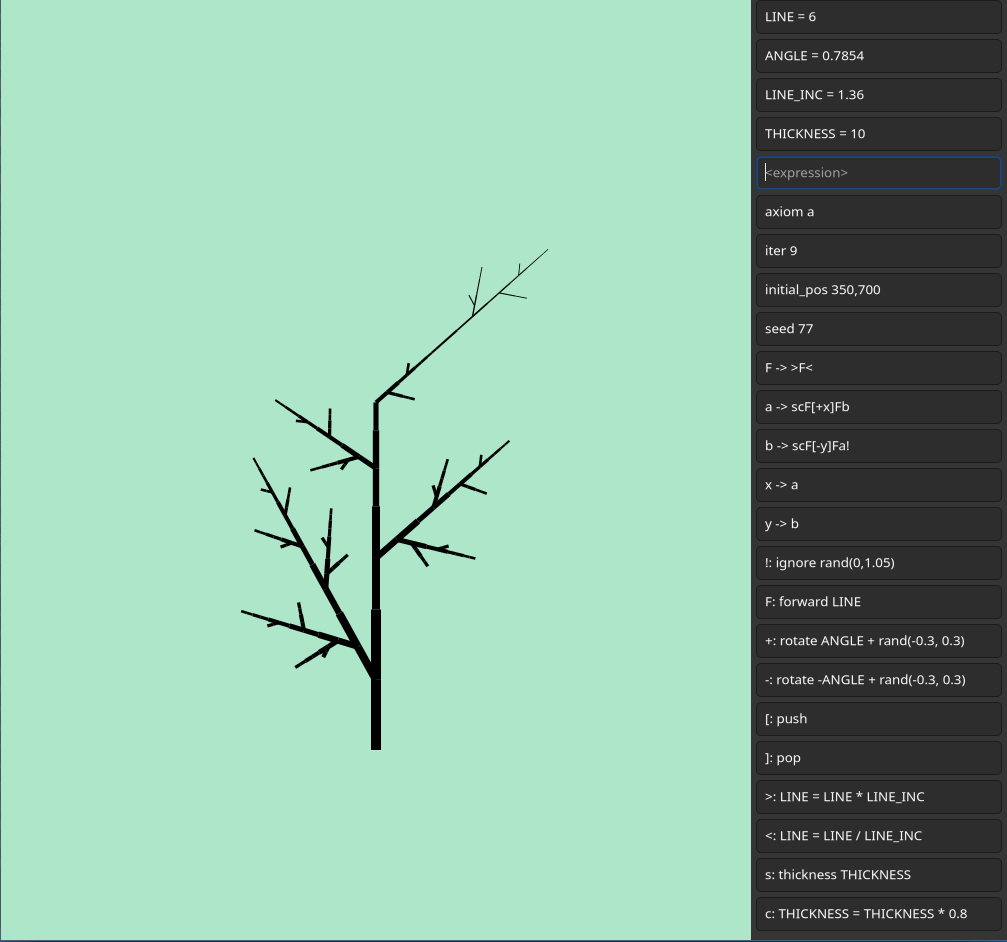
\includegraphics[width=0.8\textwidth]{fractal_ignore.png}
    \end{figure}
\end{center}

I also fixed some bugs, implemented the \texttt{canvas} command
to se the canvas size, the \texttt{initial\_thickness}
and the \texttt{initial\_pos} command.

\textbf{Git status}:
\begin{enumerate}
    \item Merged \texttt{development} into \texttt{main}
    \item Created \texttt{ignore-feature} branch
    \item Merged \texttt{ignore-feature} into \texttt{main}
    \item Created \texttt{thickness} branch
    \item Merged \texttt{thickness} into \texttt{main}
    \item Created \texttt{development} branch (generic improvements and fixes)
    \item Merged \texttt{Development} into \texttt{main}
    \item Created \texttt{logging} branch
\end{enumerate}

The plan for the next working session is to continue the documentation and maybe
some GUI editor improvements.

\subsection{2023-05-10}

Work hours:\\
\textbf{09:10 - 12:30}: GUI Editor \\
\textbf{13:10 - 14:15}: GUI Editor \\
\textbf{14:15 - 14:45}: Status label \\
\textbf{14:45 - 16:30}: Documentation

Today I continued developing the GUI editor.
\\
The various configuration textboxes are now separated into their own
retractable section. If a textbox contains an incorrect line
it will be colored red. Lines put in a different section than the one
they should be put in (e.g. a variable in the rules section)
will also produce an error. \\
The config section is hardcoded; there is a specific textbox
for the \texttt{axiom}, \texttt{iter} and so on.

I also added a status label which tells the user if an error has occured
(e.g. a variable or functioned used does not exist).

The editor does not yet create/remove empty texboxes when needed.

In the remaining time I continued the documentation.
I only modified the \texttt{Implementation} section.

\textbf{Git status}:
\begin{enumerate}
    \item Created \texttt{better-ui} branch
    \item Merged \texttt{better-ui} into \texttt{main}
    \item Merged \texttt{logging} into \texttt{main}
\end{enumerate}

I am in line with the planning.

\pagebreak

\subsection{2023-05-11}

Work hours:\\
\textbf{08:40 - 09:50}: Color feature \\
\textbf{10:10 - 11:20}: Refactor

Today I implemented the color feature. \\
A symbol may change the color of the line by using the \texttt{color <color>} operation.
Any valid CSS color is a valid color.
\\ I also added the \texttt{initial\_color <color>} command.

In the second half of the working session I refactored some code.
I had some problems with the memory management and GTK4.

In the next working session I will implement the dynamic editor behavior, namely
creating or removing textboxes as needed. \\
I will also start implementing the animation system.

\textbf{Git status}:
\begin{enumerate}
    \item Created \texttt{color-feature} branch
    \item Merged \texttt{color-feature} into \texttt{main}
\end{enumerate}

I am in line with the planning, expect for the dynamic editing feature which should have been implemented within today.

\subsection{2023-05-12}

Work hours:\\
\textbf{08:20 - 13:40}: Animation features

Today I started implementing the animations feature. \\
I had to refactor some code in order to be able to host this feature. \\
I was able to make a basic draw loop and animate the fractal, while keeping
the same random seed to something changes between frames. \\
When the configuration of the fractal changes the animation is reset. \\
I have yet to add a play/resume button and the \texttt{frame} variable
to the mathematical expressions.

This feature is very difficult to implement and I had some problems with the
memory management.

\textbf{Git status}:
\begin{enumerate}
    \item Created \texttt{animations} branch
\end{enumerate}

\subsection{2023-05-15}

Work hours:\\
\textbf{09:10 - 11:10}: UI Playback and fixes \\
\textbf{11:10 - 13:45}: Refactor \\
\textbf{13:45 - 14:00}: Depth feature \\
\textbf{14:00 - 14:50}: Optimization \\
\textbf{14:50 - 16:20}: Injections

Today I implemented the UI playback.
In the GUI I added:
\begin{itemize}
    \item A toggle button to play/stop the animation
    \item A button to reset the animation (frame=0)
    \item A counter for the current frame
    \item The elapsed time between each render
\end{itemize}

I also added the following hardcoded variables

\begin{itemize}
    \item \textbf{FRAME}: The current frame count
    \item \textbf{DEPTH}: The current stack depth
    \item \textbf{INDEX}: The current index in the fractal string
    \item \textbf{LENGTH}: The length of the fractal string
\end{itemize}

I did a lot of refactor and separated a lot of logic
into its own file. I fixed some bugs and optimized the program
overall.

I am also almost done with the \texttt{injections}
features, but the parser is still broken.

\subsection{2023-05-16}

Work hours:\\
\textbf{08:20 - 09:15}: Injections \\
\textbf{09:20 - 09:50}: Logging \\
\textbf{10:05 - 11:20}: Dynamic entries

Today I finished implementing the injections features. \\
Injections can be made using the command \texttt{inject}. \\
E.g. \texttt{inject 0,FF 100,! 1000,+F-F}

I implemented a simple terminal logger
and added a label under the canvas containing the length
of the fractal string.

I also added some logic to add new empty textboxes
if needed. The removal of them has yet to be implemented.

\textbf{Git status}:
\begin{enumerate}
    \item Merged \texttt{injections} into \texttt{main}
    \item Created \texttt{logging} branch
    \item Merged \texttt{logging} into \texttt{main}
    \item Created \texttt{dynamic-inputs} branch
\end{enumerate}

The only feature left is the \texttt{import/export} of l-system files. \\
The plan is to finish the code this week, and only document in the next one.

\subsection{2023-05-16}

\textbf{09:10 - 16:10}: Import/Export

Today I implemented the import/export buttons. \\
The export works but the import doesn't, although the logic is there.

Everything is basically done and I will finish the code in the next
working section. There are still a couple of small improvements
that could be made. \\
I will then spend the rest of the last week to complete the documentation.

\textbf{Git status}:
\begin{enumerate}
    \item Merged \texttt{dynamic-inpzts} into \texttt{main}
    \item Created \texttt{import-export} branch
\end{enumerate}

\subsection{2023-05-22}

\textbf{09:10 - 16:10}: Minor features and improvements

Today I finished implementing the application.
I implemented many small features and improvements, namely
\begin{enumerate}
    \item Added a variable \texttt{TIME}.
    \item Bug fixes.
    \item Better error label message.
    \item Added a \textbf{Clear} button.
    \item Finished the import feature.
    \item Added \texttt{jump} operation.
    \item Added \texttt{dot} operation.
    \item Added \texttt{background} command.
\end{enumerate}

Everything was easy to implement and
I fortunately did not have any problem in doing so.

Here's a picture of the final product
\begin{center}
    \begin{figure}[h]
        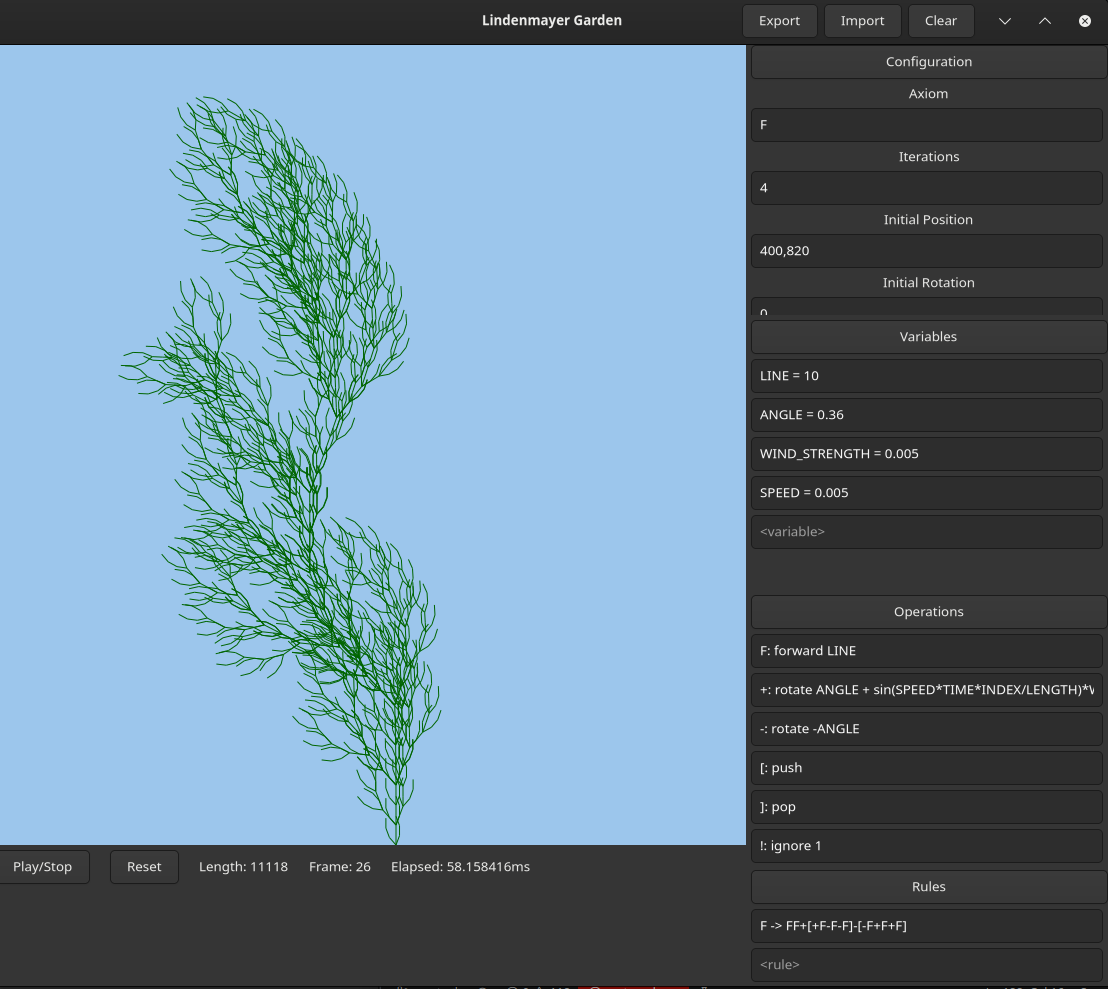
\includegraphics[width=0.7\textwidth]{final.png}
    \end{figure}
\end{center}

In the remaining time I continued the \texttt{Semantics}
subsection of the documentation.

\textbf{Git status}:
\begin{enumerate}
    \item Merged \texttt{import-export} into \texttt{main}
    \item Created \texttt{development} branch
    \item Merged \texttt{development} into \texttt{main}
\end{enumerate}

I am still ahead of planning and the documentation
is the only thing left to do.

\subsection{2023-05-23}

\textbf{08:20 - 11:10}: Documentation

Today I continued the \texttt{Implementation} section of the documentation.

I found two minor bugs in the code and easily fixed them. I also added a
\texttt{Time} label to the UI.

Half of the documentation is done, I should be able to finish it in time.
The major remaining part of the documentation is the testing cases and the implementation.

\subsection{2023-05-24}

\textbf{09:05 - 10:05}: Final Gantt Chart \\
\textbf{10:05 - 16:20}: Documentation

Today I continued the documentation.
I added the final gantt chart and wrote my considerations about it.

I continued the implementation, added references, testing section and some generic changes.

I also created the abstract file.

The documentation is almost done and I should be able to finish it tomorrow.
I mainly need to finish the implementation section and the introductory section about L-Systems.

\subsection{2023-05-25}

\textbf{08:25 - 11:15}: Documentation

Today I almost completed the documentation. I completly rewrote the \texttt{L-Systems}
sections. I fixed some typos and added some content throughout the documentation.
There are still a couple of things missing from the \texttt{Implementation},
which I will add tomorrow.

I also wrote the abstract page and everything is almost done.

\subsection{2023-05-26}

\textbf{08:20 - 11:35}: Documentation

Today I finished the documentation.
I fixed some typos and added some content in various sections.
I added the glossary and submitted my project.

\end{document}